% World models for control across the representation spectrum.
% A single combined report merging the two repository tracks:
%   (I)  R2-Dreamer transfer on DMC vision   (was reports/r2dreamer_report.tex)
%   (II) DINO-WM reproduction + low-data adaptation + local/global planning
%        (was reports/dino_wm_report.tex, which itself merged the local/global addendum)
%
% Every figure is an existing committed output under reports/figures/.
% Build: tectonic world_models_report.tex   (or pdflatex, twice)

\documentclass[11pt,a4paper]{article}

\usepackage[margin=2.5cm]{geometry}
\usepackage{amsmath,amssymb}
\usepackage{booktabs}
\usepackage{tabularx}
\usepackage{graphicx}
\usepackage{xcolor}
\usepackage{enumitem}
\usepackage{tikz}
\usetikzlibrary{arrows.meta,positioning}
\usepackage[colorlinks=true,linkcolor=blue!55!black,citecolor=blue!55!black,urlcolor=blue!55!black]{hyperref}
\usepackage{microtype}  % character protrusion + font expansion: cleaner spacing, fewer overfull lines
\graphicspath{{figures/}}
\emergencystretch=3em  % absorb residual long-typewriter-token line breaks

% Shared notation across the two tracks.
\newcommand{\zlat}{\mathbf{z}}
\newcommand{\xloc}{\mathbf{x}}
\newcommand{\act}{\mathbf{a}}
\newcommand{\abar}{\bar{\mathbf{a}}}

\title{World Models for Control across the Representation Spectrum:\\
Transfer and Planning with R2-Dreamer and DINO-WM\\
under a Commodity-GPU Budget}
\author{Thomas Georges\thanks{Engineering and experiment automation developed with
Claude (Anthropic) in the \texttt{World\_Models\_LAS} repository. Track~I code:
\texttt{scripts/r2dreamer}, \texttt{configs/r2dreamer}; Tracks~II--III code:
\texttt{src/wm\_poc/dino\_wm}, \texttt{src/wm\_poc/local\_global}. Every number
and figure is read from the committed outputs of the results notebooks
(06/07/08).}}
\date{June 16, 2026 --- v1.0 (combined report)}

\begin{document}
\maketitle

\begin{abstract}
We study how to \emph{obtain} and how to \emph{use} a world model for control
under a strict commodity-GPU budget, at two opposite choices of latent
representation. In the first track, a reconstruction-free,
representation-regularized DreamerV3 variant (``R2-Dreamer''~\cite{r2dreamer,dreamerv3})
\emph{learns} its latent end-to-end, and we measure transfer on a visual
locomotion shift on the DeepMind Control Suite~\cite{dmc}
(\texttt{walker\_walk}\,$\rightarrow$\,\texttt{walker\_run} from $64{\times}64$
pixels). In the second, DINO-WM~\cite{dinowm2025} \emph{inherits} a frozen
self-supervised representation (DINOv2 patch features~\cite{dinov2}) and learns
only an action-conditioned dynamics predictor; we reproduce it on PointMaze,
add a low-data adaptation study, and build a coupled local/global planning study
on the resulting model. The two tracks bracket the representation axis ---
learn-your-own versus inherit-frozen --- and the engineering thread that makes
both feasible on free Colab hardware is shared (a $\approx\!21\times$
latent-cache speedup is what makes the DINO-WM study runnable at all). Across
both ends \emph{two findings recur}. (i)~\textbf{Fine-tuning beats training from
scratch at equal target-task budget, at both ends} --- though \emph{what} the
warm start tests differs: Track~I is a genuine task shift
(\texttt{walker\_walk}$\rightarrow$\texttt{walker\_run}), where R2-Dreamer
reaches $742$ vs $563$ episodic return ($+32\%$, with a ${\sim}4\times$
mid-training lead and a near-zero-shot $\sim\!375$ vs $\sim\!25$ warm start);
Track~II is same-domain low-data adaptation (a full-data PointMaze checkpoint
adapted on $300$ target rollouts), where the adapted predictor delivers
$2.75\times$ the scratch baseline's real-environment planning success ($0.275$ vs
$0.10$; episode-level $z{=}4.5$, $p<10^{-5}$, not a run-level test --- all runs
are seed~0), reaches a planning score similar to the full-data checkpoint under
this evaluation, and converges in a single epoch. (ii)~\textbf{The scalar metric the model is
trained on systematically understates a structural difference in the latent
that actually governs control}: two same-task R2-Dreamer policies occupy
distinct, near-linearly-separable latent basins (the fine-tune traces a
limit-cycle manifold, scratch collapses to a blob); two DINO-WM predictors with
the \emph{same order of magnitude} of latent-prediction MSE differ $2.75\times$
in planning success;
and a local surrogate whose one-step disagreement with the global model is only
${\approx}0.002$ nonetheless yields gradient directions reliable enough to be
accepted just $2.8\%$ of the time. On the planner side, a global re-score gate
keeps cheap first-order refinement \emph{bounded-worsening} under the global
model's objective (rejecting any refinement that worsens it by more than
$\tau{=}0.05$), and here recovers global-CEM-quality plans ($0.97$ success)
where an unguarded hybrid collapses to $0.54$, while purely local planners run
$100$--$1000\times$ cheaper per episode. All results
are single-seed and at fixed budgets; we state the resulting limits throughout.
\end{abstract}

\section{Introduction}
\label{sec:intro}

A world model is useful for control to the extent that planning or acting
against it produces behavior that succeeds in the real environment. Two design
questions dominate the cost of getting there: \emph{what representation does the
model's dynamics operate over}, and \emph{how is that model adapted to a new
task}. This report collects the two experimental tracks of the
\texttt{World\_Models\_LAS} repository, which were built to probe exactly those two
questions from opposite ends, and unifies them into a single study.

\subsection{The representation spectrum, and the logic of the two tracks}
\label{sec:spectrum}

World models for control sit on a spectrum defined by \emph{where the
representation comes from} (Figure~\ref{fig:spectrum}). At one end, the model
\textbf{learns its own latent} jointly with the dynamics --- the DreamerV3
lineage~\cite{dreamer,dreamerv2,dreamerv3}, here in its reconstruction-free
R2-Dreamer form, which replaces the pixel decoder with a redundancy-reduction
representation objective~\cite{barlow}. At the other end, the model
\textbf{inherits a frozen, pretrained representation} and learns only how it
evolves under actions --- DINO-WM~\cite{dinowm2025}, which trains an
action-conditioned transition model over frozen DINOv2 patch
features~\cite{dinov2} and never updates the encoder. The first buys a
control-shaped latent at the cost of learning perception from scratch; the
second buys data- and compute-efficiency and cross-task reuse at the cost of a
representation it cannot adapt.

\begin{figure}[t]
\centering
\begin{tikzpicture}[font=\small,
  box/.style={draw,rounded corners,align=center,inner sep=5pt},
  trk/.style={box,fill=blue!5,text width=5.2cm},
  syn/.style={box,fill=green!7,text width=12.6cm},
  ar/.style={-{Latex[length=2.2mm]},semithick}]
% spectrum axis
\draw[ar,gray!75] (-6.4,0) -- (6.4,0);
\draw[ar,gray!75] ( 6.4,0) -- (-6.4,0);
\node[align=center,font=\small\bfseries] at (-4.6,0.34) {learn the representation};
\node[align=center,font=\small\bfseries] at ( 4.6,0.34) {inherit a frozen representation};
\node[gray!55!black,font=\footnotesize] at (0,-0.32) {representation axis};
% track boxes
\node[trk] (t1) at (-4.0,2.15) {\textbf{Track~I — R2-Dreamer}\\[1pt]
  DreamerV3 RSSM; reconstruction-free Barlow latent (\emph{end-to-end learned}).\\
  DMC vision, \texttt{walk}$\rightarrow$\texttt{run}.};
\node[trk] (t2) at ( 4.0,2.15) {\textbf{Track~II — DINO-WM}\\[1pt]
  frozen DINOv2 patch features; ViT dynamics predictor (\emph{only dynamics learned}).\\
  PointMaze goal reaching.};
\draw[ar] (t1.south) -- (-4.0,0.18);
\draw[ar] (t2.south) -- ( 4.0,0.18);
% synthesis box
\node[syn] (s) at (0,-2.35) {\textbf{Shared questions} \;(cross-track synthesis, \S\ref{sec:synthesis}; planning, Track~III, \S\ref{sec:trackiii})\\[2pt]
  (1)~Does fine-tuning/pretraining beat training from scratch \emph{at equal target-task budget} (Track~I: task transfer; Track~II: same-domain low-data adaptation)?\quad
  (2)~What does a planner actually consume --- the scalar training metric, or the latent's \emph{structure}?\\[1pt]
  \emph{Track~III:} plan efficiently against the trusted (expensive) DINO-WM model using a cheap differentiable surrogate, gated by a global re-score.};
\draw[ar] (-4.0,-0.18) -- (s.north west);
\draw[ar] ( 4.0,-0.18) -- (s.north east);
\end{tikzpicture}
\caption{The logic of the repository. The two experimental tracks bracket the
representation axis: R2-Dreamer learns its latent end-to-end (Track~I,
\S\ref{sec:tracki}); DINO-WM inherits a frozen DINOv2 latent and learns only
dynamics (Track~II, \S\ref{sec:trackii}). Both are then asked the same two
questions, and a third track (\S\ref{sec:trackiii}) studies efficient planning
against the DINO-WM model. The cross-track synthesis (\S\ref{sec:synthesis})
shows that the same two answers hold at both ends.}
\label{fig:spectrum}
\end{figure}

Reading the tracks side by side is the point of this report. \emph{What
transfers} differs completely --- Track~I fine-tunes an entire learned model
including its representation; Track~II fine-tunes only a dynamics predictor over
a representation that is shared and frozen --- yet, as \S\ref{sec:synthesis}
shows, the two ends agree on the answers to both shared questions. That
agreement, obtained from genuinely different machinery, is the strongest claim
the combined study can make.

\subsection{The commodity-GPU constraint}
\label{sec:constraint}

Every experiment here was built under one hard practical rule: it must run end
to end on the hardware actually available to us (Google Colab --- predominantly
a free-tier T4; an A100 only occasionally), and the experiment \emph{definition}
(model size, data budgets, episode counts, seeds) must be identical across GPU
tiers, with only throughput knobs (precision, dataloader workers, micro-batch
or rollout-chunk size, wall-clock caps) differing. This constraint turned out
to be the technically interesting part of Track~II: the stock DINO-WM loop is
not merely slow on a T4 but structurally infeasible, projecting more than
$30$ hours per epoch regardless of batch size. Diagnosing and removing that
cost \emph{without altering the experiment} (\S\ref{sec:cache}) is what makes
the Track~II results obtainable at all, and the same discipline ---
pristine-upstream checkouts with reversible runtime patches, hardware-only
profiles, and resumable stages --- runs through both tracks (\S\ref{sec:method-shared}).

\subsection{Contributions}
\label{sec:contributions}

\begin{enumerate}[leftmargin=1.5em,itemsep=2pt]
\item \textbf{(Track~I)} A faithful, budget-feasible R2-Dreamer transfer study
  on DMC vision (\S\ref{sec:tracki}): a competent \texttt{walker\_walk} world
  model gives a near-zero-shot head start on \texttt{walker\_run} and a clean
  sample-efficiency advantage over scratch at a fixed A100 budget, together with
  a latent-geometry analysis showing the fine-tuned model lands in a distinct,
  better-structured representational basin.
\item \textbf{(Track~II)} A latent-cache training path for DINO-WM that removes
  the dominant data-path cost while preserving the upstream training
  distribution for the selected windows ($\approx\!21\times$ faster, \S\ref{sec:cache}); a resumable
  PointMaze reproduction; a low-data adaptation study (scratch vs.\ fine-tune)
  with both latent-prediction and real-environment planning metrics; and the
  observation that latent-prediction loss and planning success
  \emph{dissociate} sharply (\S\ref{sec:trackii}).
\item \textbf{(Track~III)} A coupled local/global planning study on the trained
  DINO-WM model (\S\ref{sec:trackiii}): six planners spanning zero-order global
  search to first-order local optimization, with the result that a global
  re-score gate keeps first-order refinement \emph{bounded-worsening} under the
  global model's objective --- recovering global-CEM quality where an unguarded
  hybrid collapses --- while purely local planners are $100$--$1000\times$
  cheaper per episode.
\item \textbf{(Synthesis)} A cross-track reading (\S\ref{sec:synthesis})
  establishing that, at both ends of the representation spectrum, (a)~fine-tuning
  dominates scratch at equal target-task budget, and (b)~the scalar training metric
  understates a structural latent difference --- basin geometry, plannability,
  or gradient reliability --- that governs downstream control. We argue this is
  a concrete methodological warning for world-model evaluation.
\end{enumerate}

\subsection{A unifying thesis}
\label{sec:thesis}

Stated once, so the rest of the report can refer back to it: \emph{across both
ends of the representation spectrum, fine-tuning from a related-task checkpoint
(Track~I) or a full-data checkpoint (Track~II) is a large sample-efficiency win
at equal target-task budget in these single-seed runs, and the scalar quantity a world
model is trained to minimize (episodic return, latent-prediction MSE,
one-step surrogate error) is a weak proxy for the latent structure that a
controller actually consumes.} The two tracks were designed and run
independently; that they converge on the same two statements is the result.

\section{Background and related work}
\label{sec:background}

\paragraph{Latent world models and imagination.} The DreamerV3
lineage~\cite{dreamer,dreamerv2,dreamerv3} learns a Recurrent State-Space
Model (RSSM)~\cite{planet} --- a deterministic recurrent state plus a stochastic
latent --- and trains an actor--critic ``in imagination'' on rollouts of the
learned dynamics rather than on environment frames~\cite{dreamer}. Track~I uses
this backbone. PlaNet~\cite{planet} plans directly in a learned latent;
TD-MPC2~\cite{tdmpc2} pairs a learned latent model with sampling-based MPC.

\paragraph{Reconstruction-free representation objectives.} Standard Dreamer
learns its latent through pixel reconstruction with a decoder. A
reconstruction-free family removes the decoder and learns the representation
through self-supervised auxiliary losses: DreamerPro~\cite{dreamerpro} with
prototypical representations, contrastive CPC/InfoNCE~\cite{cpc}, and
Barlow-Twins-style redundancy reduction~\cite{barlow}. R2-Dreamer (Track~I)
uses the Barlow objective on projected latents; a practical consequence is that
the model has \emph{no decoder} and therefore no imagined-frame visualization.

\paragraph{Frozen self-supervised features for control.} The opposite design
freezes a powerful pretrained encoder and learns dynamics on top of its
features. DINOv2~\cite{dinov2} provides such features; the JEPA world-model
family (V-JEPA~2~\cite{vjepa2}) and DINO-WM~\cite{dinowm2025} plan over them.
DINO-WM is the concrete, planning-focused instance reproduced in Tracks~II--III:
it encodes each frame to frozen DINOv2 patch tokens, trains a transformer
predictor with a latent-consistency objective, and plans by sampling-based
optimization of latent goal distance with no decoder in the loop.

\paragraph{Sampling-based and first-order planning.} The cross-entropy method
(CEM)~\cite{cem} optimizes action sequences from forward rollouts only and is
the planner reproduced in Tracks~II--III. First-order (gradient-based) planners
are sample-efficient per iteration but require a differentiable model;
differentiable MPC~\cite{diffmpc} differentiates through the optimizer itself.
The coupled local/global idea~\cite{fog2026} resolves the accuracy-vs-
differentiability tension by letting a large trusted model produce trajectories
(never differentiated) while a lightweight surrogate supplies derivatives
evaluated along those trajectories; Track~III transplants this into DINO-WM
latent planning.

\bigskip
\noindent\emph{We now present the two tracks in turn (\S\ref{sec:tracki},
\S\ref{sec:trackii}--\S\ref{sec:trackiii}), then read them together
(\S\ref{sec:synthesis}). Notation common to the DINO-WM tracks is introduced in
\S\ref{sec:trackii}.}

% =====================================================================
\section{Track~I --- R2-Dreamer: transfer with a learned representation}
\label{sec:tracki}
% =====================================================================

Track~I is a faithful, budget-feasible demonstration of the canonical Dreamer
transfer experiment --- train a latent world model on a source task, save and
reload it, adapt it to a shifted task, and compare fine-tuning against scratch
--- using the \emph{representation-regularized} R2-Dreamer objective on image
observations. The three-way comparison is
\[
\begin{aligned}
\texttt{source\_base} &:~\texttt{walker\_walk}~\text{(from scratch)},\\
\texttt{target\_finetune} &:~\texttt{walker\_run}~\text{(initialized from \texttt{source\_base})},\\
\texttt{target\_scratch} &:~\texttt{walker\_run}~\text{(from scratch)},
\end{aligned}
\]
all on \texttt{dmc\_vision} ($64\times64$ RGB), orchestrated from a single Colab
notebook against an unmodified upstream checkout.\footnote{\texttt{NM512/r2dreamer}~\cite{r2dreamer},
a PyTorch reimplementation of DreamerV3~\cite{dreamerv3} extending
\texttt{NM512/dreamerv3-torch}~\cite{dreamerv3torch}; behavioral changes are
applied as marker-guarded, idempotent, reversible textual patches at launch
time (\S\ref{sec:method-shared}).}

\subsection{Model}
\label{sec:tracki-model}

\paragraph{Backbone.} A DreamerV3-style latent world model: a convolutional
encoder maps each $64{\times}64{\times}3$ frame to an embedding; an
RSSM~\cite{planet} carries a deterministic recurrent state and a stochastic
latent and predicts forward dynamics; reward and continuation heads decode task
quantities; and an actor--critic is trained entirely in imagination. The
observation is vision only (no proprioceptive MLP input).

\paragraph{Representation objective (the ``R2'').} The upstream code exposes a
swappable representation loss (\texttt{model.rep\_loss} $\in$ \{\texttt{dreamer},
\texttt{r2dreamer}, \texttt{infonce}, \texttt{dreamerpro}\}). We use
\texttt{r2dreamer}: a reconstruction-free objective that learns the
representation through a projector head trained with a redundancy-reduction
(Barlow-Twins-style) loss on projected latents~\cite{barlow}, placing it in the
same reconstruction-free family as DreamerPro~\cite{dreamerpro} and CPC/
InfoNCE~\cite{cpc}. The \texttt{r2dreamer} model has \emph{no decoder}: there is
no imagined-frame path, so visual analysis uses environment-rendered policy
rollouts and the geometry of the RSSM latent states, not decoded
reconstructions.

\paragraph{Parameter budget.} The \texttt{size25M} configuration instantiates
$26.53$M trainable parameters, dominated by the RSSM and the R2 projector head
(Table~\ref{tab:tracki-model}). Each checkpoint is $325.9$\,MB (fp32 weights
plus Adam moments).

\begin{table}[h]
\centering\small
\begin{tabular}{lrl}
\toprule
Component & Parameters & Role \\
\midrule
RSSM               & 13{,}442{,}304 & latent dynamics (recurrent + stochastic state) \\
Projector          &  5{,}898{,}240 & R2 representation head (redundancy reduction) \\
Value (critic)     &  1{,}869{,}951 & imagined-return value \\
Actor (policy)     &  1{,}776{,}396 & imagination policy \\
Reward predictor   &  1{,}573{,}503 & reward head \\
Continue predictor &  1{,}475{,}713 & episode-continuation head \\
Encoder (CNN)      &    493{,}824 & $64\times64\times3 \rightarrow$ embedding \\
\midrule
\textbf{Total}     & \textbf{26{,}529{,}931} & \\
\bottomrule
\end{tabular}
\caption{R2-Dreamer components and parameter counts (read from the extraction
logs of notebook~06).}
\label{tab:tracki-model}
\end{table}

\subsection{Setup and resources}
\label{sec:tracki-setup}

Source task \texttt{dmc\_walker\_walk}, target \texttt{dmc\_walker\_run}, both
$64{\times}64$ RGB. The fine-tune run initializes \emph{all} world-model weights
from the source checkpoint with a strict state-dict load and does \emph{not}
carry over optimizer state (\texttt{pretrained\_strict=true},
\texttt{load\_optimizer=false}); scratch is identical except for random
initialization. Both target runs share a $400$k-step budget, so the comparison
is at equal target experience (Table~\ref{tab:tracki-config}). Training and
analysis ran on a single NVIDIA~A100 (Colab), Python~3.11, with the DMC tasks on
MuJoCo~\cite{mujoco,dmcontrol}; image observations are produced by headless
OSMesa rendering while the policy runs on CUDA.

\begin{table}[h]
\centering\small
\begin{tabular}{ll@{\hspace{1.4em}}ll}
\toprule
Setting & Value & Setting & Value \\
\midrule
Observation        & \texttt{dmc\_vision} $64{\times}64{\times}3$ & Train ratio   & 224 \\
Model              & \texttt{size25M}                            & Parallel envs & 8 \\
Representation loss & \texttt{r2dreamer} (Barlow-style)          & Eval cadence  & every 50k steps, 5 episodes \\
Batch              & 16 sequences $\times$ length 64             & Seed          & 0 \\
Source steps       & 800k (reached $\sim$796k)                   & Target steps  & 400k (reached $\sim$396k) \\
\bottomrule
\end{tabular}
\caption{Track~I configuration (the \texttt{a100\_r2\_vision25m} three-way preset).}
\label{tab:tracki-config}
\end{table}

\subsection{Results}
\label{sec:tracki-results}

\begin{table}[h]
\centering\small
\begin{tabular}{llrrrr}
\toprule
Run & Init & Task & Final eval & Final train & Env steps \\
\midrule
\texttt{source\_base}     & random            & \texttt{walker\_walk} & $968.3$ & $964.2$ & $\sim$796k \\
\texttt{target\_finetune} & \texttt{source\_base} & \texttt{walker\_run}  & $742.3$ & $693.4$ & $\sim$396k \\
\texttt{target\_scratch}  & random            & \texttt{walker\_run}  & $563.1$ & $529.7$ & $\sim$396k \\
\bottomrule
\end{tabular}
\caption{Final results (DMC episodic return, $0$--$1000$). ``Eval'' is the
deterministic 5-episode score; ``train'' the rolling training return. For all
three runs the best eval equals the final eval (no late-training collapse).}
\label{tab:tracki-results}
\end{table}

\paragraph{Source task is effectively solved.} The source model reaches
evaluation return $968.3$ on \texttt{walker\_walk} (the DMC walk reward saturates
near $1000$), so the checkpoint we fine-tune from is a competent walker --- the
prerequisite for a meaningful transfer test. Figure~\ref{fig:tracki-source}
shows the monotone climb to that ceiling.

\begin{figure}[h]
\centering
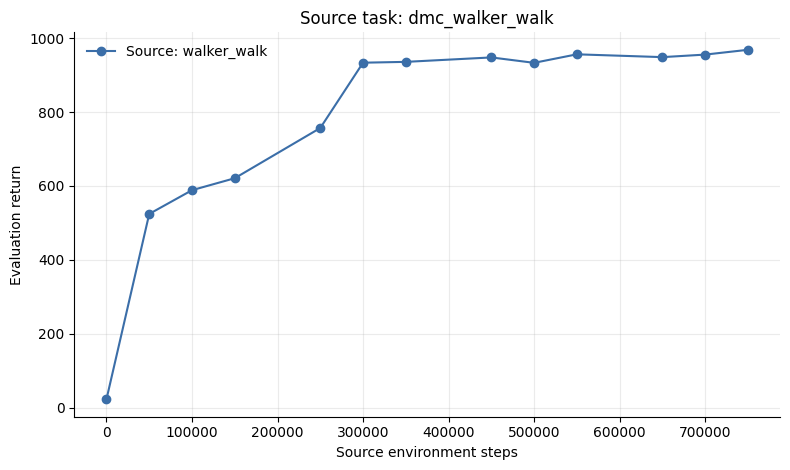
\includegraphics[width=0.58\linewidth]{r2dreamer_source_eval_curve.png}
\caption{Source-task evaluation return over $\sim$796k steps: \texttt{walker\_walk}
converges to $\approx\!968$, providing the fine-tune initialization.}
\label{fig:tracki-source}
\end{figure}

\paragraph{Transfer dominates scratch at every budget.} This is the central
Track~I result (Figure~\ref{fig:tracki-transfer}). Three features stand out.
\emph{(i)~A large warm start:} at the first evaluation, before any run-specific
gradient steps, the fine-tuned policy already returns $\sim\!375$ on
\texttt{walker\_run} versus $\sim\!25$ for random scratch --- walk and run share
enough locomotion structure to transfer almost zero-shot. \emph{(ii)~Faster
convergence:} by $100$k target steps the fine-tune is at $\sim\!600$ while
scratch is near $\sim\!150$, a ${\sim}4\times$ gap; the fine-tune passes $700$
by $\sim$300k. \emph{(iii)~A persistent but shrinking lead:} the fine-tune ends
at $742$ and scratch at $563$, a $+179$ ($+32\%$) advantage at the shared
$400$k budget. The advantage curve starts at $\sim\!352$, peaks at $\sim\!448$
around $100$k steps, and declines steadily as the scratch baseline --- still
rising at the budget limit --- closes part of the gap. The result therefore
demonstrates \emph{sample efficiency}, not necessarily a higher asymptotic
ceiling (\S\ref{sec:limits}).

\begin{figure}[h]
\centering
\begin{minipage}{0.49\linewidth}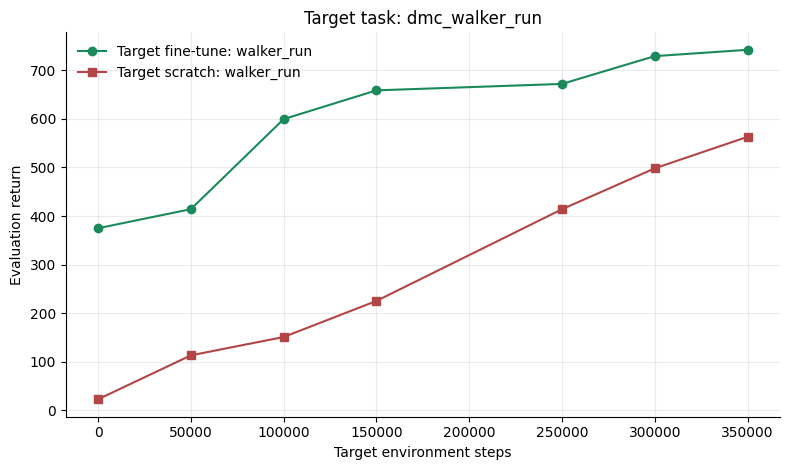
\includegraphics[width=\linewidth]{r2dreamer_target_eval_curve.png}\end{minipage}\hfill
\begin{minipage}{0.49\linewidth}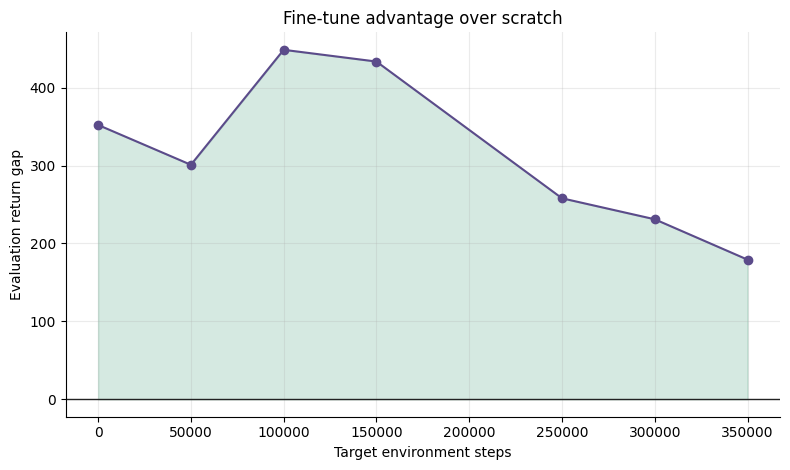
\includegraphics[width=\linewidth]{r2dreamer_finetune_advantage.png}\end{minipage}
\caption{Target-task transfer. \textbf{Left:} evaluation return on
\texttt{walker\_run}, fine-tune (green) vs.\ scratch (red); fine-tune leads at
every evaluation. \textbf{Right:} step-aligned advantage (fine-tune $-$ scratch),
peaking at $\sim\!448$ near $100$k steps and declining to $+179$ at the budget
limit.}
\label{fig:tracki-transfer}
\end{figure}

\paragraph{Training dynamics and optimization health.} The training-episode
curves (Figure~\ref{fig:tracki-train}, left) reveal a brief adaptation
transient: the fine-tune begins near $\sim\!400$ (inherited walk competence),
\emph{dips} to $\sim\!270$ as the gait is repurposed for running --- a short,
recoverable negative-transfer phase --- then climbs steadily past scratch.
Optimization is stable for all three runs
(Figure~\ref{fig:tracki-train}, right): every loss component descends and stays
bounded, and the R2-specific Barlow redundancy-reduction term drops sharply and
flattens, indicating the reconstruction-free objective trained as intended.

\begin{figure}[h]
\centering
\begin{minipage}{0.46\linewidth}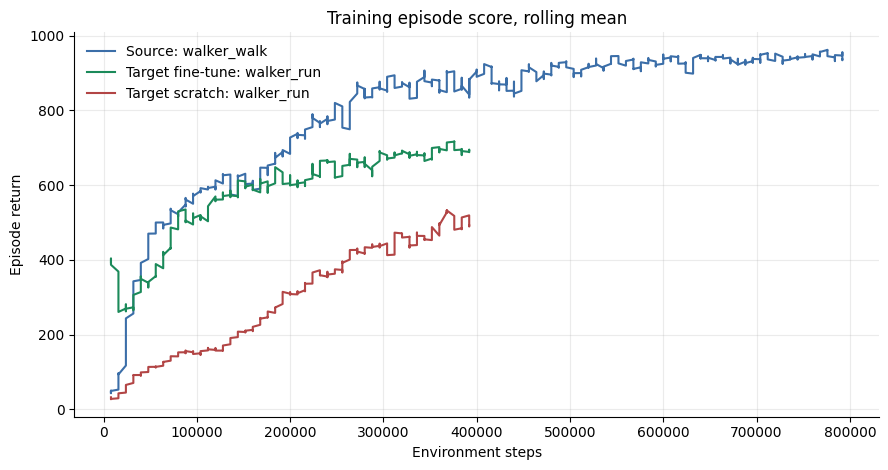
\includegraphics[width=\linewidth]{r2dreamer_training_episode.png}\end{minipage}\hfill
\begin{minipage}{0.52\linewidth}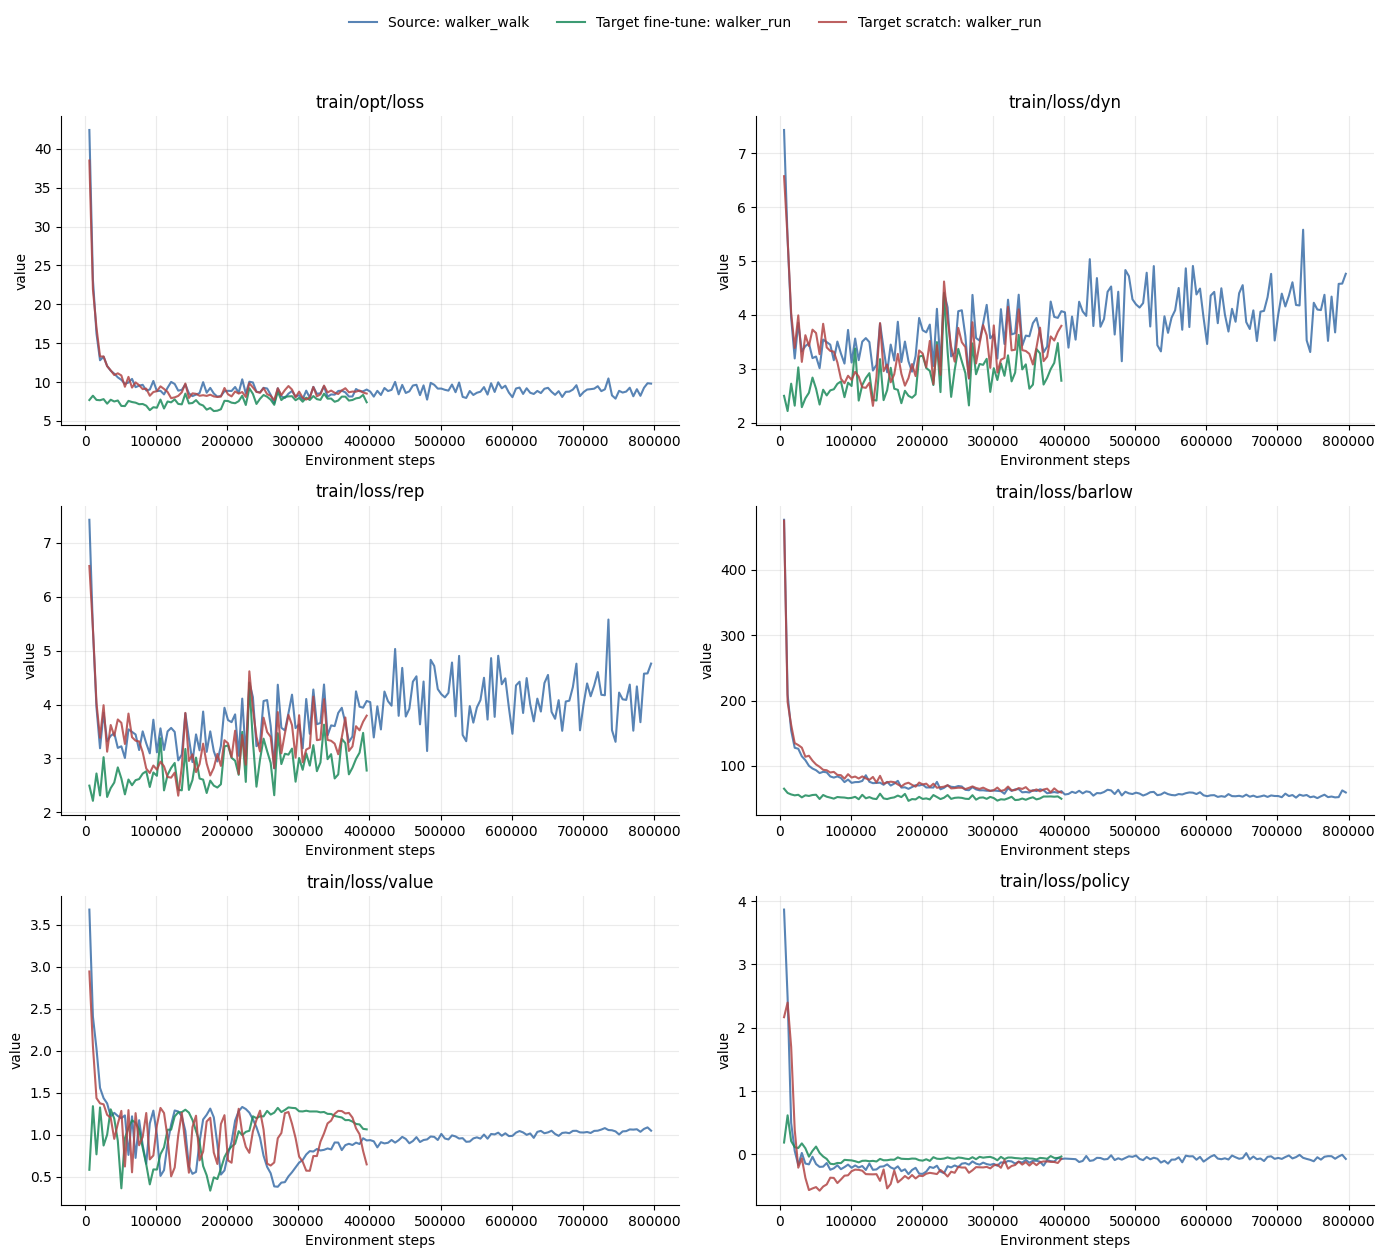
\includegraphics[width=\linewidth]{r2dreamer_diagnostics.png}\end{minipage}
\caption{\textbf{Left:} rolling-mean training episode return (window~8): source
(blue) to $\sim\!950$; fine-tune (green) starts high, dips during gait
re-adaptation, converges near $\sim\!690$; scratch (red) rises from near zero to
$\sim\!530$, still increasing. \textbf{Right:} optimization diagnostics --- all
loss components bounded and convergent, including \texttt{train/loss/barlow}.}
\label{fig:tracki-train}
\end{figure}

\paragraph{Latent geometry: the two policies live in different basins.} We
extracted RSSM recurrent features along three evaluation episodes ($1500$ states
each) for the fine-tune and scratch \texttt{walker\_run} policies and projected
them with a shared-basis PCA (Figure~\ref{fig:tracki-pca}). Although both solve
the \emph{same} task, their latent states occupy clearly separated regions ---
near-linearly separable along PC1 --- so the warm-started model encodes the task
\emph{differently}, not merely faster. The 3D view is more striking: the
fine-tuned model's latents trace a large, organized ring/limit-cycle manifold
consistent with a periodic running gait, whereas the scratch model's latents
collapse into a small, compact cluster, mirroring its lower return. The top
three components explain only $\approx\!9.5/3.8/3.5\%$ of the variance
($\sim\!17\%$ total), so these projections capture the dominant linear structure,
not the full latent geometry (\S\ref{sec:limits}). This geometric difference,
which the scalar return only partly conveys, is the first instance of the
report's second thesis (\S\ref{sec:synthesis}).

\begin{figure}[h]
\centering
\begin{minipage}{0.42\linewidth}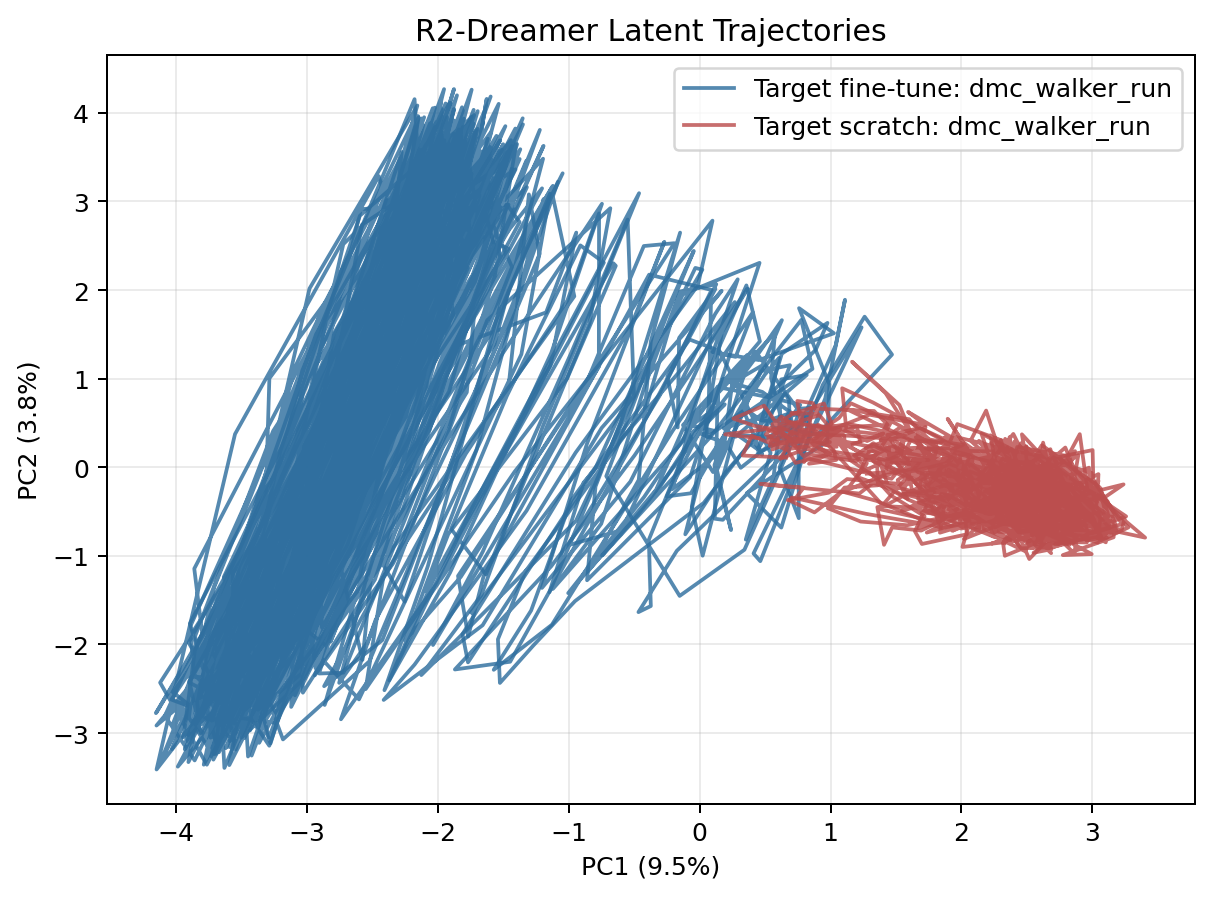
\includegraphics[width=\linewidth]{r2dreamer_latent_pca_2d.png}\end{minipage}\hfill
\begin{minipage}{0.55\linewidth}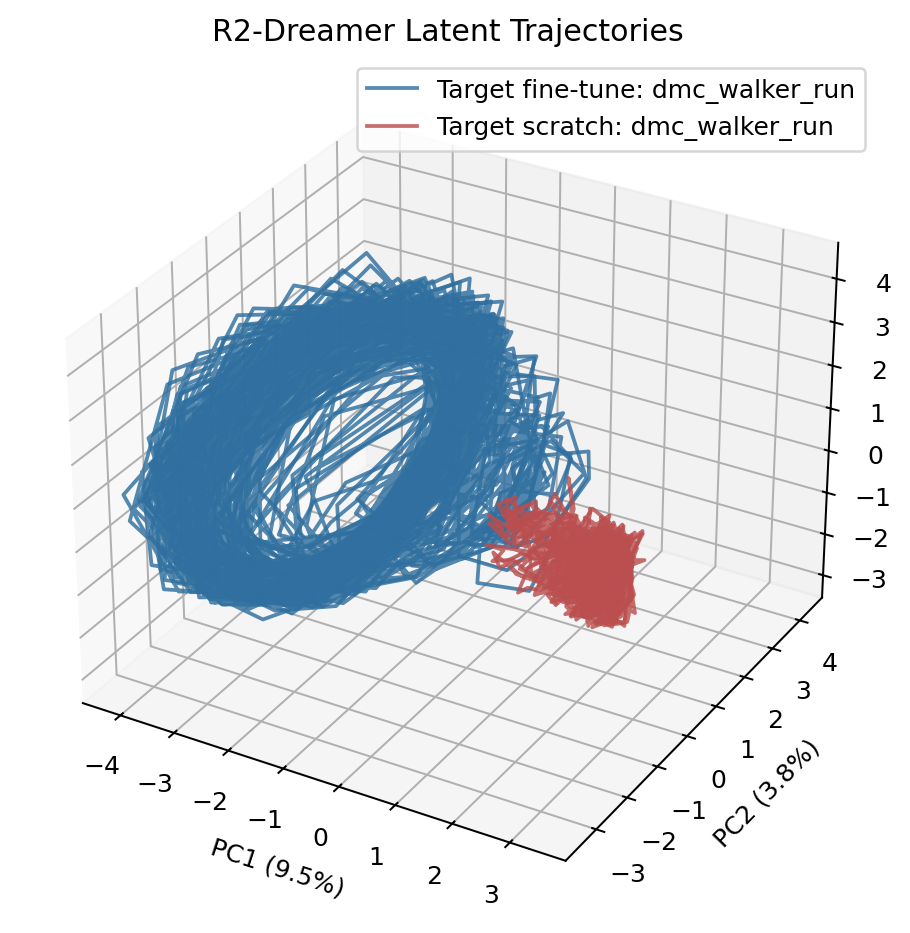
\includegraphics[width=\linewidth]{r2dreamer_latent_pca_3d.png}\end{minipage}
\caption{Shared-basis PCA of RSSM latent trajectories, fine-tune (blue) vs.\
scratch (red) on \texttt{walker\_run}. \textbf{Left (2D):} separation along PC1.
\textbf{Right (3D):} the fine-tune traces a large cyclically structured
manifold; scratch occupies a compact blob.}
\label{fig:tracki-pca}
\end{figure}

The results notebook (06) also renders one environment-camera rollout per
checkpoint plus a rotating 3D latent-PCA animation; because the model is
decoder-free these are true renderings of the executed policy, and their
qualitative content tracks Table~\ref{tab:tracki-results} (a near-solved walk, a
competent fine-tune run, a weaker scratch run).

% =====================================================================
\section{Track~II --- DINO-WM: planning with a frozen representation}
\label{sec:trackii}
% =====================================================================

Track~II reproduces DINO-WM~\cite{dinowm2025} on PointMaze under the commodity-GPU
constraint of \S\ref{sec:constraint}, and uses it for a low-data adaptation study
that mirrors Track~I's question at the frozen-representation end of the spectrum.

\paragraph{Notation.} PointMaze episodes are frame sequences with raw 2-D
actions $\act_t \in [-1,1]^2$ and proprioception. Following DINO-WM, one
\emph{model step} advances $f$ raw steps (frameskip $f{=}5$); the model-step
action is the folded block
$\abar_k = [\act_{kf};\dots;\act_{(k+1)f-1}] \in \mathbb{R}^{fA}$. Each frame is
encoded to $\zlat \in \mathbb{R}^{P\times D}$ with $P{=}196$ patches and
$D{=}384$ (DINOv2 ViT-S/14 at $224$\,px, a $14{\times}14$ patch grid). The
predictor consumes $H{=}3$ context frames and predicts the next latent
(\texttt{num\_pred}=1). Episode-level train/validation splits are drawn from a
seeded permutation of the \emph{uncapped} episode count, so split membership is
invariant to how many rollouts a run uses.

\subsection{The DINO-WM model as reproduced}
\label{sec:trackii-model}

\paragraph{Encoder (frozen).} \texttt{dinov2\_vits14}, feature key
\texttt{x\_norm\_patchtokens}, frozen throughout (\texttt{train\_encoder=false}),
with the upstream preprocessing transform. \textbf{Predictor:} a ViT
(\texttt{models.vit.ViTPredictor}; depth 6, 16 heads, MLP width 2048, dropout
0.1) over the flattened $H{\times}P = 3{\times}196 = 588$ token sequence.
Actions and proprioception are embedded ($10{+}10$) and concatenated along the
feature axis (\texttt{concat\_dim}=1), giving working dimension
$D{+}10{+}10 = 404$; a causal temporal mask is applied. \textbf{Objective:}
with $\hat{\zlat}$ the predicted next latent and $\zlat$ the detached target,
\begin{equation}
\mathcal{L} \;=\; \big\lVert \hat{\zlat} - \mathrm{sg}[\zlat] \big\rVert_2^2 ,
\label{eq:trackii-loss}
\end{equation}
the latent-consistency MSE, reported per epoch as a training and a validation
(``h-step'') component. The runs are \emph{decoder-free}
(\texttt{has\_decoder=false}): no pixel reconstruction is trained, which halves
memory and matches the planning objective (planning never decodes).

\subsection{Feasible training: the latent-cache path}
\label{sec:cache}

\paragraph{Why the stock loop costs $>$30\,h/epoch.} Profiling identified three
compounding causes, none addressable by batch size (confirmed: batch~4 and
batch~32 both project ${\sim}19$--$21$\,h/epoch on a T4). \emph{(1)~Per-sample
episode reload:} upstream \texttt{TrajSlicerDataset} fetches a 4-frame window by
\texttt{torch.load}-ing the \emph{entire} episode ($\sim$93 frames) and
transforming every frame, then discarding all but four; at ${\sim}147$k
windows/epoch this re-reads ${\sim}1600\times$ the dataset per epoch through the
Drive FUSE mount. \emph{(2)~Online re-encoding of frozen features:} with
\texttt{train\_encoder=false} the DINOv2 outputs are dataset constants, yet
every frame of every window is re-encoded every epoch --- pure recomputation.
\emph{(3)~Operational confounders:} single-threaded loading and reads from Drive
rather than local disk.

\paragraph{Encode once, reuse forever.} Because the encoder is frozen, its
outputs can be precomputed. Three marker-guarded patches, installed at launch:
\emph{(1)~one-time precompute} --- each episode is read once, preprocessed
\emph{exactly} as upstream, encoded under autocast, and written as a per-episode
\texttt{fp16} \texttt{.npy} plus a manifest (${\sim}30$\,GB for all $2200$
episodes, on session-local disk; idempotent and resumable); \emph{(2)~a drop-in
latent dataset} selected by Hydra override that subclasses the upstream dataset,
so actions, states, proprioception, normalization, and the seeded split are
\emph{bit-identical} to the online path by construction (the subclass overrides
only the visual features; \texttt{scripts/dino\_wm/validate\_latent\_cache.py}
checks the split, manifest, latent shape, dtype, and planning-path dispatch),
memory-mapping only
the ${\sim}0.6$\,MB of latents each window needs instead of a ${\sim}13$\,MB
episode; \emph{(3)~an input-dispatch bypass} in \texttt{encode\_obs} (4-D latent
inputs skip the encoder; 5-D image inputs take the original path), so planning,
which encodes real observations, is untouched. For the selected windows this
preserves the upstream split, actions, proprioception, normalization, and the
planning-time image-encoding path exactly --- the only thing that changes is
when and how often the frozen (\texttt{fp16}-cached) encoder runs. The one
deliberate departure is the full T4 run's stride-2 window subsampling
(Table~\ref{tab:throughput}), a throughput-biased lower-bound experiment rather
than a paper-exact schedule (\S\ref{sec:limits}); the low-data pair uses the full
stride-1 set.

\begin{table}[h]
\centering\small
\begin{tabularx}{\linewidth}{@{}Xrrrr@{}}
\toprule
Configuration & Steps/epoch & Step time (T4) & Epoch (T4) & Epoch (A100, est.) \\
\midrule
Stock, batch 4                   & 36{,}815 & $\sim$3\,s    & $>$30\,h          & --- \\
Stock, batch 32                  & 4{,}602  & 15.9--17\,s   & 19--21\,h (proj.) & --- \\
Latent cache, batch 32, stride 1 & 4{,}602  & $\sim$0.76\,s & $\sim$58\,min     & 6--12\,min \\
Latent cache, batch 32, stride 2 & 2{,}330  & 0.72--0.76\,s & 31\,min (meas.)   & 3--6\,min \\
\bottomrule
\end{tabularx}
\caption{Training throughput before and after the latent-cache path
($\approx\!21\times$). The residual step cost is the depth-6 ViT predictor
itself --- the quantity the experiment is meant to measure. ``Stride 2''
subsamples window starts and was used only for the full run on T4; the low-data
pair uses the full stride-1 set.}
\label{tab:throughput}
\end{table}

\subsection{Planning and evaluation}
\label{sec:trackii-planning}

Planning uses the upstream CEM~\cite{cem}/MPC path unchanged. Given start and
goal observations, CEM optimizes an open-loop action sequence to minimize the
predicted latent distance to the goal encoding:
\begin{equation}
J(\abar_{1:H}) \;=\; \tfrac{1}{PD}\big\lVert \hat{\zlat}_H(\abar_{1:H}) - \zlat_{\mathrm{goal}} \big\rVert_2^2 ,
\label{eq:trackii-objective}
\end{equation}
iterating sample/score/refit (population 100, 10 iterations, goal horizon
$G{=}5$, \texttt{goal\_source\allowbreak =random\_state}). Crucially, while CEM
\emph{optimizes} an imagined latent quantity, \textbf{success is measured in the
real MuJoCo environment}: the planned actions are executed and success is the
environment's own goal-reaching test. Reported success rates are therefore real
closed-loop control outcomes, not the model's self-assessment.

\subsection{Runs}
\label{sec:trackii-runs}

Three runs enter the results (Table~\ref{tab:trackii-runs}); all train the
predictor only, on cached latents, with identical seeds, normalization, and
splits. Precision is bf16 on A100/L4 and fp16 on T4; all runs are seed~0. CEM
population/iters $100/10$, $200$ planning evaluations per checkpoint.

\begin{table}[h]
\centering\small
\begin{tabular}{@{}lllll@{}}
\toprule
Run & Data (train+val) & Epochs & Initialization & Planning evals \\
\midrule
Full no-decoder    & 2000 + 200 & 10 & random          & 200 \\
Low-data scratch   & 300 + 60   & 30 & random          & 200 \\
Low-data fine-tune & 300 + 60   & 20 & full checkpoint & 200 \\
\bottomrule
\end{tabular}
\caption{Runs. Fine-tuning loads the predictor and action/proprio encoders from
the full run's checkpoint and continues at reduced learning rates
($10^{-5}$/$10^{-4}$); the frozen DINOv2 encoder is shared. The full run was
trained on a T4 with stride-2 window subsampling (Table~\ref{tab:throughput}).}
\label{tab:trackii-runs}
\end{table}

\subsection{Results}
\label{sec:trackii-results}

All numbers are read from the \emph{latest} \texttt{final\_eval} row of each
run's planner \texttt{logs.json}, at 200 evaluation episodes per checkpoint
(Wilson half-width ${\approx}0.06$).

\paragraph{Training loss: fine-tuning starts where scratch ends.} The fine-tuned
predictor attains at \emph{epoch~1} the validation loss the scratch baseline
reaches only after ${\sim}30$ epochs (Figure~\ref{fig:trackii-curves}):
pre-training delivers the converged predictor for ${\sim}30\times$ fewer
updates on the low-data task. The honest caveat is that scratch \emph{does}
converge to the same order of magnitude by epoch~30
(Figure~\ref{fig:trackii-scratchft}: $\approx\!0.021$ vs $\approx\!0.012$) ---
which makes the planning result that follows all the more pointed.

\begin{figure}[h]
\centering
\begin{minipage}{0.62\linewidth}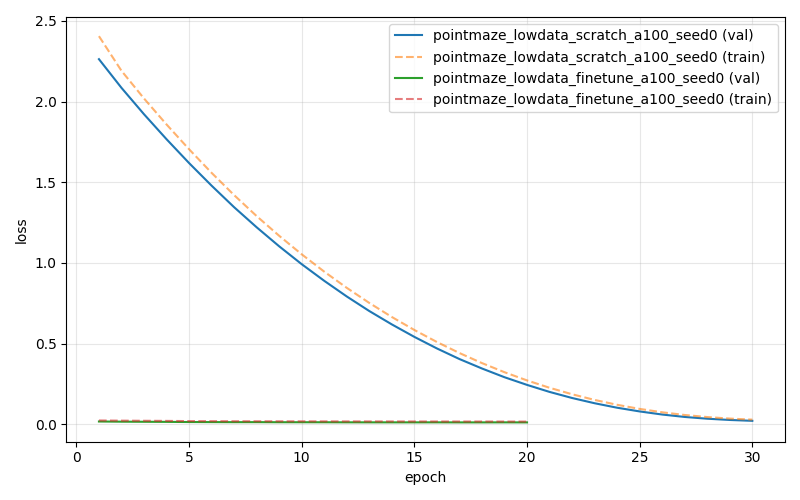
\includegraphics[width=\linewidth]{pointmaze_training_curves.png}\end{minipage}\hfill
\begin{minipage}{0.36\linewidth}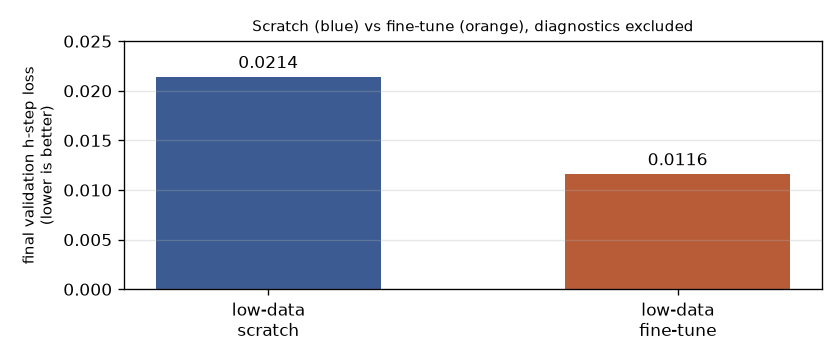
\includegraphics[width=\linewidth]{pointmaze_scratch_vs_finetune.png}\end{minipage}
\caption{\textbf{Left:} per-epoch training (dashed) and validation (solid)
latent-prediction loss. Scratch descends from $\approx\!2.3$ to $\approx\!0.02$
over 30 epochs; the fine-tune begins at $\approx\!0.015$ at epoch~1 --- already
the scratch run's converged level --- and stays there. \textbf{Right:} final
validation h-step loss, scratch vs.\ fine-tune ($\approx\!0.021$ vs
$\approx\!0.012$, same order of magnitude).}
\label{fig:trackii-curves}
\label{fig:trackii-scratchft}
\end{figure}

\paragraph{Planning success in the real environment.} At $n{=}200$ the Wilson
intervals tighten to $\pm0.06$ (Figure~\ref{fig:trackii-success}). Two clean
results stand out. \textbf{Fine-tune $\boldsymbol{>}$ scratch} is decisive
($0.275$ vs $0.10$; an episode-level two-proportion $z{=}4.5$, $p<10^{-5}$ --- a
Bernoulli approximation over the 200 evaluation episodes, not a run-level test,
since all runs are seed~0): pre-training on the full corpus and adapting on 300
rollouts yields $2.75\times$ the planning success of training on those same 300
rollouts from scratch.
\textbf{Fine-tune vs.\ full-data} ($0.275$ vs $0.23$) is statistically
indistinguishable ($p{=}0.30$): a full-data-pretrained predictor, adapted on 300
target rollouts, reaches a similar 200-episode planning score to the full-data
checkpoint under this evaluation. The full model's $0.23$ is moreover a lower
bound (T4 stride-2 subsampling, half the gradient updates of the paper-exact
stride-1 set); an A100 stride-1 run is needed to test whether the full-data
score improves under the paper-exact window schedule. (The larger sample moved
all three estimates down from the noisier 50-eval interim,
$0.34/0.26/0.12 \to 0.275/0.23/0.10$, without disturbing the ranking.)

\begin{figure}[h]
\centering
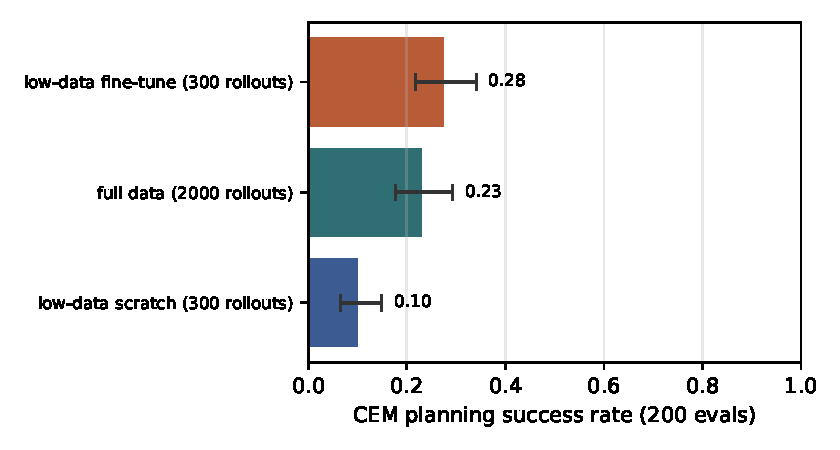
\includegraphics[width=0.66\linewidth]{success_rates.pdf}
\caption{Closed-loop CEM planning success in MuJoCo PointMaze, 200 evaluation
episodes per checkpoint, 95\% Wilson intervals: fine-tune $0.275$, full-data
$0.23$, scratch $0.10$.}
\label{fig:trackii-success}
\end{figure}

\paragraph{The loss/planning dissociation.} The central empirical finding of
Track~II is the contrast between Figure~\ref{fig:trackii-scratchft} and
Figure~\ref{fig:trackii-success}: scratch and fine-tune converge to the same
order of magnitude in validation latent-prediction loss ($\approx\!0.021$ vs
$\approx\!0.012$) yet differ $2.75\times$ in real-environment planning success
($0.10$ vs $0.275$, $p<10^{-5}$). The scalar loss alone does not rank downstream
control quality: this ${\sim}2\times$ residual loss gap (same order of magnitude)
coincides with a near-tripling of planning success, which points to additional
geometric or calibration differences that the scalar MSE does not capture --- the
fine-tuned model's latent geometry appears more \emph{plannable} (smoother or
better-calibrated for CEM) despite a similar average prediction error. The practical
consequence is direct: \emph{a planning metric must be carried alongside the
loss curve}; the loss alone would have reported these two models as equivalent.
This is the second instance of the report's second thesis
(\S\ref{sec:synthesis}).

\paragraph{Planner diagnostics: CEM is genuinely optimizing.} The
per-iteration telemetry (Figure~\ref{fig:trackii-cem}) confirms CEM is
exploiting the learned dynamics rather than stumbling onto goals: environment
success of the current best plan rises and mean state distance falls
monotonically over the 10 iterations for every trained model, with scratch
improving least. The embedding-divergence panel shows the better models keep
imagination closest to executed reality at the end of optimization --- exactly
the property a planner needs.

\begin{figure}[h]
\centering
\begin{minipage}{0.33\linewidth}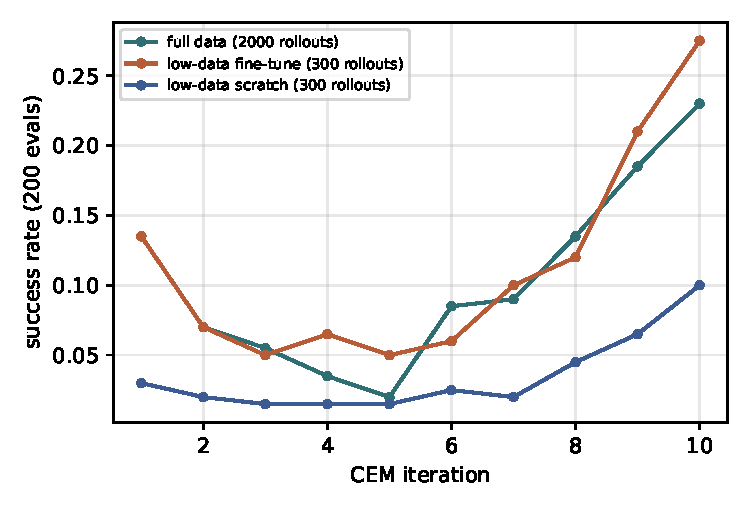
\includegraphics[width=\linewidth]{cem_success.pdf}\end{minipage}\hfill
\begin{minipage}{0.33\linewidth}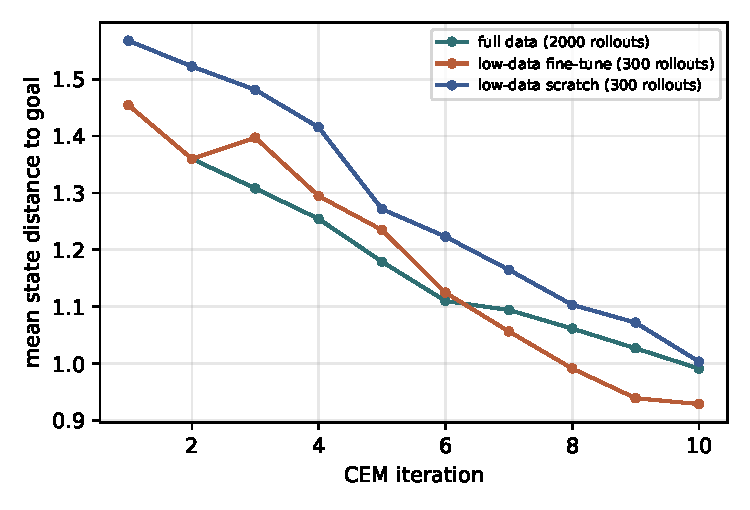
\includegraphics[width=\linewidth]{cem_state_dist.pdf}\end{minipage}\hfill
\begin{minipage}{0.33\linewidth}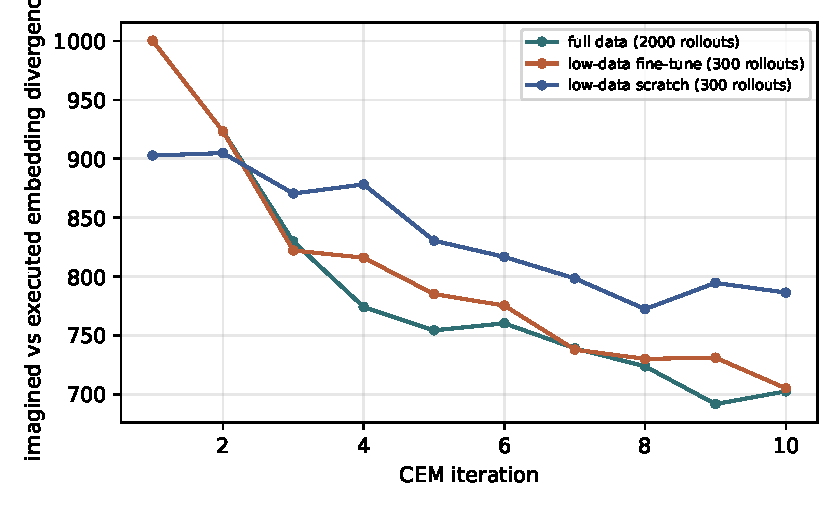
\includegraphics[width=\linewidth]{cem_embed_div.pdf}\end{minipage}
\caption{Planner-internal telemetry per CEM iteration (exact values from
\texttt{logs.json}). \textbf{Left:} environment success of the current best plan
rises across the 10 iterations (full $0.135\!\to\!0.23$; fine-tune
$0.135\!\to\!0.275$; scratch $0.03\!\to\!0.10$). \textbf{Middle:} mean state
distance to goal falls correspondingly (fine-tune $1.45\!\to\!0.93$).
\textbf{Right:} imagined-vs-executed embedding divergence --- the model's own
rollout error; the fine-tune and full models keep imagination closest to
reality.}
\label{fig:trackii-cem}
\end{figure}

% =====================================================================
\section{Track~III --- Coupled local/global planning on the DINO-WM model}
\label{sec:trackiii}
% =====================================================================

The trained DINO-WM checkpoint (\S\ref{sec:trackii}) is the \emph{global} model
for a second study: cheap first-order planning against a trusted,
non-differentiated world model~\cite{fog2026}. Zero-order planners (CEM) work
with any accurate forward model but scale poorly in horizon and action
dimension; first-order planners are sample-efficient per iteration but need a
differentiable model --- and a model small enough to differentiate cheaply is
usually inaccurate enough to be \emph{exploited}, with gradient descent walking
into regions where it is wrong. The coupled recipe decouples the two roles: the
large model produces trajectories and is never differentiated, while a
lightweight \emph{local} surrogate supplies derivatives evaluated \emph{along
the global model's trajectories}. We instantiate it on the PointMaze DINO-WM
model and ask whether first-order refinement through a cheap surrogate can
recover global-CEM-quality plans at a fraction of the global-model compute.

\subsection{Method}
\label{sec:trackiii-method}

The \textbf{global model} is the frozen DINO-WM latent predictor, used as
forward simulator and scorer under \texttt{no\_grad}. The \textbf{local model}
is a small residual-MLP surrogate
$\xloc_{k+1} = \xloc_k + g_\theta([\xloc_k;\abar_k])$ (width 512, 3 layers) over
a \emph{frozen} orthogonal projection $\xloc = W_{\!p}\,\mathrm{pool}(\mathrm{LN}(\zlat))
\in \mathbb{R}^{256}$ of the same latents, differentiable in the actions and
trained on cached transitions. Freezing the projection is principled: a jointly
trained projector admits the degenerate optimum $W_{\!p}{=}0$ (representation
collapse), whereas a frozen near-orthogonal projection of LayerNormed features
preserves distances (Johnson--Lindenstrauss) and removes the collapse mode. Six
\textbf{planners} are compared: \texttt{global\_cem} (zero-order on the global
model); \texttt{local\_cem}, \texttt{local\_gd}, \texttt{local\_adam}
(zero/first-order on the surrogate alone, isolating model error from optimizer
effects); \texttt{hybrid\_cem\_local\_refine} (global CEM, then local
first-order refinement of the winning sequence); and
\texttt{hybrid\_cem\_local\_refine\_global\_rescore} (the same, but the global
model re-scores the refinement and rejects it only if it \emph{worsens} the
global objective by more than a relative tolerance $\tau{=}0.05$ --- a
bounded-worsening gate, so a refinement up to $\tau$ worse is still accepted).
Three safeguards against
surrogate exploitation are built in --- the frozen projection (anti-collapse),
an action-smoothness penalty, and the global re-score gate --- and the
local--global \emph{disagreement} (surrogate prediction vs.\ the global model's
executed step) is logged throughout.

\subsection{Protocol and its stated bias}
\label{sec:trackiii-protocol}

Planners are scored on offline latent goal reaching over $100$ held-out
episodes: normalized final distance
$\rho=\lVert\zlat_{\mathrm{fin}}-\zlat_{\mathrm{goal}}\rVert^2/
\lVert\zlat_{\mathrm{start}}-\zlat_{\mathrm{goal}}\rVert^2$ and
$\text{success}=\mathbb{1}[\rho<0.5]$. \textbf{Because the global model is both
simulator and judge}, \texttt{global\_cem} is structurally favored on distance
--- it optimizes exactly the quantity it is scored on --- so the
distance/success columns establish only that the other planners are
\emph{competent}, while the efficiency columns (wall time, forward/backward call
counts) and the acceptance rate carry the comparative claim. A \emph{reference
replay} of the dataset's true action sequence through the same simulator
calibrates the global model's own rollout error at $\rho_{\mathrm{ref}}=0.058$.

\subsection{Results}
\label{sec:trackiii-results}

The surrogate reaches a final validation one-step loss of $0.0058$ and a
$K$-step rollout MSE of $0.0029$ at $20{,}000$ steps
(Figure~\ref{fig:trackiii-rollout}). The six-planner comparison is
Table~\ref{tab:trackiii-planners}.

\begin{figure}[h]
\centering
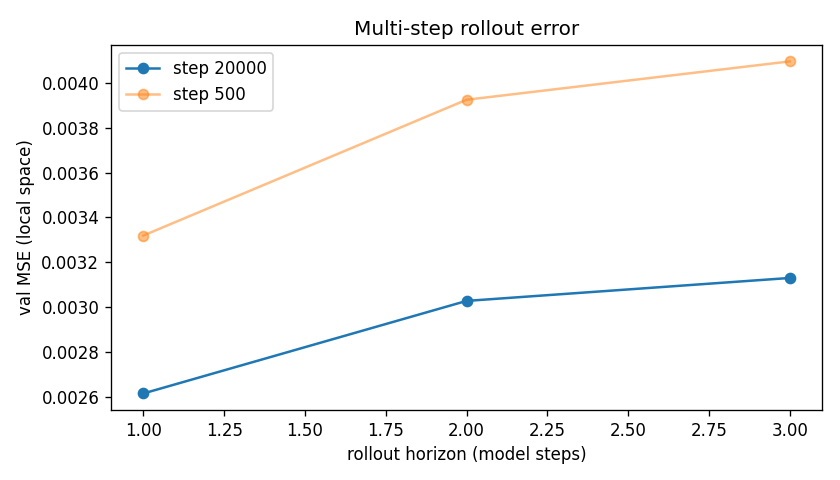
\includegraphics[width=0.52\linewidth]{pointmaze_local_full_seed0_rollout_error.png}
\caption{Surrogate validation rollout error vs.\ horizon (PointMaze, seed~0),
exported by notebook~08.}
\label{fig:trackiii-rollout}
\end{figure}

\begin{table}[h]
\centering\scriptsize
\setlength{\tabcolsep}{4pt}
\begin{tabular}{@{}lcccccccc@{}}
\toprule
Planner & succ. & $\rho$ & wall/ep.\ (s) & glob.\ fwd & loc.\ fwd & bwd & accept & disagr. \\
\midrule
\texttt{global\_cem}                     & 0.97 & 0.138 & 231.6 & 1.50M & --    & --    & --    & --     \\
\texttt{local\_cem}                      & 0.45 & 0.675 & 0.22  & --    & 1.50M & --    & --    & 0.0020 \\
\texttt{local\_gd}                       & 0.13 & 1.306 & 2.60  & --    & 50k   & 50k   & --    & 0.0028 \\
\texttt{local\_adam}                     & 0.41 & 0.699 & 2.67  & --    & 50k   & 50k   & --    & 0.0019 \\
\texttt{hybrid\_cem\_local\_refine}      & 0.54 & 0.632 & 234.1 & 1.50M & 50k   & 50k   & 1.00  & 0.0019 \\
\texttt{hybrid\_\dots\_global\_rescore}  & \textbf{0.97} & \textbf{0.138} & 234.2 & 1.50M & 50k & 50k & 0.028 & 0.0024 \\
\midrule
reference replay                         & --   & 0.058 & --    & --    & --    & --    & --    & --     \\
\bottomrule
\end{tabular}
\caption{Planner comparison on offline latent goal reaching, $100$ held-out
PointMaze episodes (surrogate at $20$k steps). Distances are judged by the
global model (see the stated bias), so the efficiency columns carry the
comparative claim. \texttt{accept}=refinement acceptance rate;
\texttt{disagr.}=mean local--global disagreement.}
\label{tab:trackiii-planners}
\end{table}

\paragraph{Findings.}
\begin{enumerate}[leftmargin=1.5em,itemsep=2pt]
\item \textbf{Global CEM tops the distance metric} ($0.97$, $\rho{=}0.138$), as
the judge bias predicts; even so its $0.138$ is ${\approx}2.4\times$ the
reference-replay floor ($0.058$) --- the global model does not perfectly close
its own gap.
\item \textbf{Pure local planners are far cheaper but weaker} on the
global-judged metric: \texttt{local\_cem} $0.45$ at \textbf{$0.22$\,s/episode},
\texttt{local\_adam} $0.41$ at $2.7$\,s, \texttt{local\_gd} $0.13$ --- against
\texttt{global\_cem}'s \textbf{$231$\,s/episode}. The surrogate forward is
${\sim}1000\times$ cheaper per call, but at this capacity it cannot plan to
global quality alone.
\item \textbf{The unguarded hybrid hurts.} \texttt{hybrid\_cem\_local\_refine}
accepts \emph{every} refinement ($\text{accept}{=}1.00$) and falls to $0.54$:
refining on the surrogate walks a good global plan into regions where the
surrogate is wrong --- the exploitation failure mode the safeguards target.
\item \textbf{The global re-score gate fixes it.}
\texttt{hybrid\_\dots\_global\_rescore} rejects $97.2\%$ of refinements
($\text{accept}{=}0.028$) and recovers global-CEM quality \emph{exactly}
($0.97$, $\rho{=}0.138$). This is the headline: the gate turns large
surrogate-exploitation failures into no-ops, so the hybrid stays bounded-worsening
under the global model's objective (within $\tau{=}0.05$ of the CEM it began
from) and here matches its quality exactly.
\item \textbf{Disagreement is small, yet gradients are unreliable.} The
local--global disagreement stays ${\approx}0.002$ --- the surrogate tracks the
global model's one-step behavior --- yet its gradient \emph{directions} improve
the global objective rarely enough that the gate accepts only $2.8\%$ of them.
One-step tracking accuracy and gradient usefulness are not the same thing --- the
third instance of the report's second thesis (\S\ref{sec:synthesis}).
\end{enumerate}

\paragraph{Synthetic sanity check.} On the exact synthetic point-mass task
(closed-form perfect global model; a few hundred surrogate steps; a correctness
signal rather than statistics) the expected ordering holds: all six planners
succeed, \texttt{local\_adam} attains the lowest final distance, the hybrids
improve on plain CEM with their refinements accepted, and \texttt{local\_gd} is
weakest. In an adversarial unit test where the surrogate's action gain is
sign-flipped, refinement reliably worsens the global cost and the re-score gate
rejects it, returning the CEM sequence unchanged.

\paragraph{What this establishes.} The protocol measures planner behavior
\emph{under the global model's belief}. It shows first-order refinement through a
cheap surrogate can be made \emph{bounded-worsening} under the global model's
objective --- rejected whenever it worsens that objective by more than
$\tau{=}0.05$ --- by a global re-score gate, and that the pure local planners are
$100$--$1000\times$ cheaper per episode. It cannot, by construction, rank planners against reality;
real-environment confirmation in MuJoCo PointMaze is the headline next step
(\S\ref{sec:future}).

% =====================================================================
\section{Cross-track synthesis}
\label{sec:synthesis}
% =====================================================================

The two tracks were designed and run independently and instantiate genuinely
different machinery --- a learned, reconstruction-free latent versus a frozen,
pretrained one; locomotion control versus goal-reaching planning. Read together,
they converge on the two statements of \S\ref{sec:thesis}.

\subsection{Fine-tuning wins at both ends of the representation spectrum}
\label{sec:synthesis-finetune}

At the \emph{learned-representation} end, fine-tuning the whole R2-Dreamer model
from \texttt{walker\_walk} gives an almost zero-shot head start on
\texttt{walker\_run} ($\sim\!375$ vs $\sim\!25$), a ${\sim}4\times$ mid-training
lead, and a $+179$ ($+32\%$) advantage at a fixed $400$k budget. At the
\emph{frozen-representation} end, fine-tuning only the DINO-WM dynamics
predictor from a full-data checkpoint converges in a single epoch (${\sim}30\times$
fewer updates) and yields $2.75\times$ the scratch baseline's real-environment
planning success ($0.275$ vs $0.10$), reaching a planning score similar to the
full-data checkpoint. \emph{What} transfers is entirely different --- an entire
model including its representation, versus a dynamics head over a shared frozen
latent --- but the qualitative answer is the same: at equal target-task budget,
warm-starting (from a related task in Track~I, from a full-data checkpoint in
Track~II) is a large sample-efficiency win, and in both tracks the scratch
baseline had not closed the gap within the budget studied.

\subsection{The scalar fit is not the usable structure}
\label{sec:synthesis-structure}

The sharper shared finding is that the scalar quantity each model is trained to
minimize understates a \emph{structural} difference in the latent that governs
downstream behavior (Table~\ref{tab:synthesis}). In Track~I, the $+32\%$ return
gap accompanies a \emph{qualitative} representational difference the scalar does
not convey: two policies solving the same task occupy distinct, near-linearly-
separable PCA basins, and the better one carries a limit-cycle manifold where
the worse one collapses to a blob --- fine-tuning changed \emph{what} was
learned, not just how fast. In Track~II, two predictors with latent-prediction
MSE of the \emph{same order of magnitude} differ $2.75\times$ in planning
success: similar average prediction error, unequal plannability. In Track~III, a surrogate whose
one-step disagreement with the global model is a mere ${\approx}0.002$ produces
gradient directions reliable enough to survive the re-score gate only $2.8\%$ of
the time: one-step fit does not imply usable gradients. In each case a scalar
fit/accuracy metric (return, latent-MSE, one-step error) is a weak proxy for the
latent or gradient \emph{geometry} a controller consumes --- which is why every
track had to carry a structural or downstream diagnostic (PCA geometry, a real-
environment planning metric, refinement acceptance) alongside the headline
scalar.

\begin{table}[h]
\centering\small
\setlength{\tabcolsep}{5pt}
\begin{tabular}{@{}p{2.5cm}p{3.4cm}p{3.7cm}p{4.6cm}@{}}
\toprule
\textbf{Track} & \textbf{Scalar signal (misleading)} & \textbf{What it hides} & \textbf{Diagnostic that reveals it} \\
\midrule
I — R2-Dreamer (learned latent) &
episodic return; both policies solve \texttt{walker\_run} &
the two policies encode the task in \emph{different latent basins} &
shared-basis PCA: PC1-separable; limit-cycle manifold vs.\ collapsed blob \\
\addlinespace
II — DINO-WM (frozen latent) &
validation latent-MSE $\approx\!0.012$ vs $\approx\!0.021$ (same order) &
a $2.75\times$ gap in real-environment \emph{plannability} &
closed-loop CEM success in MuJoCo (0.275 vs 0.10, $p{<}10^{-5}$) \\
\addlinespace
III — local/global (surrogate) &
one-step local--global disagreement $\approx\!0.002$ &
\emph{gradient directions} that rarely improve the global objective &
global re-score acceptance rate $=2.8\%$ \\
\bottomrule
\end{tabular}
\caption{One finding, three instances: across the spectrum, the scalar a model
is trained to fit understates a structural latent/gradient difference that
controls downstream behavior, and only a structural or downstream diagnostic
exposes it.}
\label{tab:synthesis}
\end{table}

\subsection{A shared engineering methodology}
\label{sec:method-shared}

Both tracks reach these results through the same discipline, which is itself
part of the contribution because it is what made the studies feasible and
trustworthy on free hardware. \emph{(1)~Pristine upstream, runtime patches:} all
behavioral changes (R2-Dreamer checkpoint load/save and headless-render guard;
DINO-WM latent cache, validation \texttt{no\_grad}, fine-tune init, decoder-free
video recording) are marker-guarded, idempotent, reversible textual patches
applied at launch with backups, unit-tested against the real upstream source;
neither upstream repository is vendored or edited in place. \emph{(2)~One
experiment, hardware-only profiles:} GPU-tier configs differ only in throughput
knobs (precision, dataloader workers, wall-clock caps, rollout-chunk or window
stride); model sizes, data budgets, episode counts, and run names are shared, so
a run started on one tier resumes on another. \emph{(3)~Resumability everywhere:}
per-epoch plus rolling intra-epoch checkpoints, and per-episode planning resume
(the latest \texttt{final\_eval} is authoritative), bound any disconnection to
minutes of lost work --- essential when a single sweep (e.g.\ the ${\sim}20$\,h
six-planner evaluation) exceeds a free-tier session. \emph{(4)~Smoke + unit
tests:} a ${\sim}10$--$15$\,min end-to-end smoke exercises the exact production
pipeline before any costly run, and ${\sim}95$ (DINO-WM) / ${\sim}170$
(local/global) tests cover patch composition, command rendering, run-state
gates, metrics extraction, latent-dataset parity, and analytic planner
correctness (including a sign-flipped surrogate that asserts the rejection gate
fires).

\section{Computational resources}
\label{sec:resources}

Every experiment fits inside free-tier Colab limits, with the experiment
\emph{definition} identical across GPU tiers (\S\ref{sec:constraint}); only
throughput knobs differ between a T4, an L4, and an A100. Baseline DINO-WM runs
use a free-tier T4 (16\,GB, fp16); an A100-40\,GB or L4 (bf16) is used
opportunistically. The enabling optimization is the latent cache: the stock loop
re-encodes ${\sim}1600\times$ the dataset through frozen DINOv2 every epoch,
projecting $19$--$30$\,h/epoch on a T4; precomputing the patch latents once cuts
per-step cost ${\approx}21\times$ (Table~\ref{tab:throughput}), to $31$\,min/epoch
on a T4 at stride~2 or $3$--$6$\,min on an A100. Track~I's R2-Dreamer runs use a
single A100 at a fixed $400$k-step target budget per run.

\begin{table}[h]
\centering\small
\begin{tabular}{@{}lll@{}}
\toprule
Stage & Budget & Wall-clock \\
\midrule
\multicolumn{3}{@{}l}{\emph{Track~II — DINO-WM (PointMaze)}}\\
Latent precompute (one-time)        & $2{,}200$ episodes $\to$ DINOv2     & amortized; ${\sim}30$\,GB cache \\
Predictor training, full            & $10$ epochs, $2{,}000{+}200$ traj. & ${\sim}31$\,min/epoch T4; $3$--$6$\,min A100 \\
Predictor training, low-data ($\times2$) & $20$--$30$ ep, $300{+}60$ traj. & well under the full run ($15\%$ data) \\
Planning eval (per checkpoint)      & $200$ episodes, CEM $100{\times}10$ & ${\sim}47$\,min (A100, measured) \\
\addlinespace
\multicolumn{3}{@{}l}{\emph{Track~III — local/global}}\\
Surrogate training                  & $20{,}000$ steps                   & ${\sim}1$--$2.5$\,h (T4) \\
Six-planner eval                    & $100$ episodes $\times\,6$ planners & ${\sim}20$\,h total (resumable) \\
\addlinespace
\multicolumn{3}{@{}l}{\emph{Track~I — R2-Dreamer (DMC vision)}}\\
Source / target training            & $800$k / $400$k steps, \texttt{size25M} & single A100, per run \\
\bottomrule
\end{tabular}
\caption{Wall-clock footprint on the stated hardware. The six-planner sweep is
dominated by the three planners that call the global model
(${\approx}232$--$234$\,s/episode, ${\approx}6.5$\,h per $100$ episodes) against
${\approx}0.2$--$2.7$\,s for the purely local planners --- the ${\sim}1000\times$
asymmetry that motivates the coupled design.}
\label{tab:resources}
\end{table}

\section{Threats to validity and limitations}
\label{sec:limits}

\begin{itemize}[leftmargin=1.4em,itemsep=2pt]
\item \textbf{Single seed throughout.} Every run is seed~0; there are no error
bars. The Track~I mid-training ${\sim}4\times$ gap and $+179$ final advantage,
and the Track~II $2.75\times$ planning gap ($z{=}4.5$, an episode-level Bernoulli
approximation over the 200 evaluation episodes), are large relative to typical
run-to-run noise, but run-level statistical claims would require additional seeds.
\item \textbf{Fixed budgets; scratch not converged.} The R2-Dreamer scratch
baseline is still rising at $400$k steps, so its $+179$ deficit measures sample
efficiency at a fixed budget, not an asymptotic ceiling. Likewise the DINO-WM
full model's $0.23$ is a lower bound (T4 stride-2 subsampling).
\item \textbf{Loss/planning and PCA caveats.} The Track~I PCA explains only
$\sim\!17\%$ of variance in three components, so the basin separation and ring
structure are real on the dominant axes but not the full latent geometry. The
Track~II planning estimates are $200$-episode point estimates ($\pm0.06$
Wilson).
\item \textbf{Offline local/global protocol.} Track~III judges distances with
the global model itself, so it ranks planners \emph{under the model's belief},
not against reality; the efficiency columns and acceptance rate carry the
comparative claim, and real-environment confirmation is future work.
\item \textbf{No representation-loss ablation (Track~I).} We run only
\texttt{rep\_loss=r2dreamer} and do not compare against \texttt{dreamer},
\texttt{infonce}, or \texttt{dreamerpro}, so the report characterizes \emph{this}
configuration rather than attributing the transfer result to the R2 objective
specifically. Being decoder-free, it also offers no reconstruction/imagination
metric.
\item \textbf{Precision across tiers.} T4 runs use fp16, A100/L4 bf16/TF32;
cross-tier results are statistically equivalent, not bit-identical.
\end{itemize}

\section{Conclusion and future work}
\label{sec:future}

Across two world-model designs that sit at opposite ends of the representation
spectrum --- a learned, reconstruction-free R2-Dreamer latent and a frozen,
pretrained DINO-WM latent --- and under a strict commodity-GPU budget, the same
two conclusions hold. Fine-tuning from a related-task checkpoint (Track~I) or a
full-data checkpoint (Track~II) is a large single-seed sample-efficiency win over
training from scratch at equal target-task budget in the reported fixed-budget runs; and
the scalar metric a world model is trained to minimize is a weak proxy for the
latent structure a controller consumes, so world-model evaluation must carry a
structural or downstream diagnostic alongside the loss or return. On the planner
side, a global re-score gate keeps cheap first-order refinement bounded-worsening
under the global model's scored objective --- rejecting refinements that worsen
it by more than a small tolerance --- while keeping the door open to its
$100$--$1000\times$ per-call efficiency.

The most valuable next steps are shared across tracks: \emph{(1)~seed
replication} of every headline comparison (the Track~I target pair, the Track~II
low-data pair, the Track~III sweep) to put error bars on the advantages;
\emph{(2)~extended/parity budgets} --- a longer R2-Dreamer scratch run to
separate ``head start'' from ``higher ceiling,'' and an A100 stride-1 full-data
DINO-WM training to replace the stride-2 lower bound; \emph{(3)~real-environment
confirmation} of the local/global planner ranking in MuJoCo PointMaze, the one
claim the offline protocol cannot make; \emph{(4)~ablations} --- the R2-Dreamer
representation-loss family, and the local/global projection/context/optimizer
levers and FOG-style online surrogate fine-tuning motivated by the low
acceptance rate; and \emph{(5)~harder shifts} --- Meta-World or
proprio$\rightarrow$vision transfer for R2-Dreamer, and PushT (blocked upstream
on a video-backed latent cache) for the DINO-WM tracks, where contact dynamics
should stress both the surrogate and the re-score safeguard most.

\section*{Reproducibility}

{\sloppy
Code lives in the \texttt{World\_Models\_LAS} repository. \textbf{Track~I:}
\texttt{scripts/r2dreamer}, \texttt{configs/r2dreamer}; notebook~01 trains
(Colab A100, Python~3.11, default \texttt{a100\_vision} preset) and notebook~06
regenerates results, rollout videos, and the latent analysis.
\textbf{Tracks~II--III:} \texttt{src/wm\_poc/dino\_wm} and
\texttt{src/wm\_poc/local\_global}, \texttt{scripts/dino\_wm} and
\texttt{scripts/local\_global}, \texttt{configs/dino\_wm} and
\texttt{configs/local\_global}; notebook~02 runs the DINO-WM pipeline and
notebook~03 the local/global pipeline (both self-gating and resumable, T4 or
A100), with notebooks~07/08 rendering the results. The latent-cache design is
documented in \texttt{docs/dino\_wm\_latent\_cache\_training.md} and the
local/global method in \texttt{docs/local\_global\_techniques.md}; planning
figures are produced from recorded telemetry
(\texttt{reports/pointmaze\_planning\_logs\_200evals.csv}) by
\texttt{reports/make\_planning\_figures.py}. Every figure and number in this
report is read from the committed outputs of notebooks~06/07/08.
\par}

\begin{thebibliography}{99}
\setlength{\itemsep}{2pt}

\bibitem{dreamerv3} D.~Hafner, J.~Pasukonis, J.~Ba, and T.~Lillicrap.
\emph{Mastering Diverse Domains through World Models}. arXiv:2301.04104, 2023.

\bibitem{dreamerv2} D.~Hafner, T.~Lillicrap, M.~Norouzi, and J.~Ba.
\emph{Mastering Atari with Discrete World Models}. ICLR, 2021. arXiv:2010.02193.

\bibitem{dreamer} D.~Hafner, T.~Lillicrap, J.~Ba, and M.~Norouzi.
\emph{Dream to Control: Learning Behaviors by Latent Imagination}. ICLR, 2020.
arXiv:1912.01603.

\bibitem{planet} D.~Hafner, T.~Lillicrap, I.~Fischer, R.~Villegas, D.~Ha,
H.~Lee, and J.~Davidson. \emph{Learning Latent Dynamics for Planning from
Pixels}. ICML, 2019. arXiv:1811.04551.

\bibitem{dreamerpro} F.~Deng, I.~Jang, and S.~Ahn. \emph{DreamerPro:
Reconstruction-Free Model-Based Reinforcement Learning with Prototypical
Representations}. ICML, 2022. arXiv:2110.14565.

\bibitem{barlow} J.~Zbontar, L.~Jing, I.~Misra, Y.~LeCun, and S.~Deny.
\emph{Barlow Twins: Self-Supervised Learning via Redundancy Reduction}. ICML,
2021. arXiv:2103.03230.

\bibitem{cpc} A.~van den Oord, Y.~Li, and O.~Vinyals.
\emph{Representation Learning with Contrastive Predictive Coding}.
arXiv:1807.03748, 2018.

\bibitem{dinowm2025} G.~Zhou, H.~Pan, Y.~LeCun, and L.~Pinto.
\emph{DINO-WM: World Models on Pre-trained Visual Features Enable Zero-shot
Planning}. ICML, 2025. arXiv:2411.04983.

\bibitem{dinov2} M.~Oquab, T.~Darcet, T.~Moutakanni, et al.
\emph{DINOv2: Learning Robust Visual Features without Supervision}.
Transactions on Machine Learning Research (TMLR), 2024. arXiv:2304.07193.

\bibitem{vjepa2} M.~Assran, A.~Bardes, D.~Fan, Q.~Garrido, et al.
\emph{V-JEPA 2: Self-Supervised Video Models Enable Understanding, Prediction
and Planning}. arXiv:2506.09985, 2025.

\bibitem{tdmpc2} N.~Hansen, H.~Su, and X.~Wang.
\emph{TD-MPC2: Scalable, Robust World Models for Continuous Control}. ICLR, 2024.

\bibitem{diffmpc} B.~Amos, I.~D.~J.~Rodriguez, J.~Sacks, B.~Boots, and
J.~Z.~Kolter. \emph{Differentiable MPC for End-to-end Planning and Control}.
NeurIPS, 2018.

\bibitem{fog2026} J.~Amigo, R.~Khorrambakht, N.~Mansard, and L.~Righetti.
\emph{Coupled Local and Global World Models for Efficient First-Order RL}.
arXiv:2602.06219, 2026.

\bibitem{cem} P.-T.~de Boer, D.~P.~Kroese, S.~Mannor, and R.~Y.~Rubinstein.
\emph{A Tutorial on the Cross-Entropy Method}. Annals of Operations Research,
134(1):19--67, 2005.

\bibitem{dmc} Y.~Tassa et al. \emph{DeepMind Control Suite}. arXiv:1801.00690,
2018.

\bibitem{dmcontrol} S.~Tunyasuvunakool et al.
\emph{dm\_control: Software and Tasks for Continuous Control}.
Software Impacts, 6:100022, 2020.

\bibitem{mujoco} E.~Todorov, T.~Erez, and Y.~Tassa.
\emph{MuJoCo: A Physics Engine for Model-Based Control}. IROS, 2012.

\bibitem{r2dreamer} N.~Morihira, A.~Nahar, K.~Bharadwaj, Y.~Kato, A.~Hayashi,
and T.~Harada. \emph{R2-Dreamer: Redundancy-Reduced World Models without Decoders
or Augmentation}. ICLR, 2026. arXiv:2603.18202. Code:
\url{https://github.com/NM512/r2dreamer}.

\bibitem{dreamerv3torch} NM512. \emph{dreamerv3-torch: PyTorch Implementation of
DreamerV3}. GitHub repository, \url{https://github.com/NM512/dreamerv3-torch}.

\end{thebibliography}

\end{document}
